\definecolor{cfwone}{HTML}{eef5fa}
\definecolor{cfwtwo}{HTML}{daeaf5}
\definecolor{cfwthree}{HTML}{b2d2e9}
\definecolor{cfwfour}{HTML}{8abbde}

\newcommand{\fwone}[1]{\colbox{cfwone}{#1}\xspace}
\newcommand{\fwtwo}[1]{\colbox{cfwtwo}{#1}\xspace}
\newcommand{\fwthree}[1]{\colbox{cfwthree}{#1}\xspace}
\newcommand{\fwfour}[1]{\colbox{cfwfour}{#1}\xspace}

\newcommand{\fexp}[2]{\texttt{[{\color{darkgray}{#1:#2}}]}\xspace}
\newcommand{\fexptag}[1]{\fexp{TAG}{#1}}
\newcommand{\fexpfrom}[1]{\fexp{FROM}{#1}}
\newcommand{\fexpto}[1]{\fexp{TO}{#1}}
\newcommand{\fexptemp}[1]{\fexp{TEMP}{#1}}


\section{Counterfactual Explanations}
\label{sec:app_explain}

\begin{figure}[t]
\centering
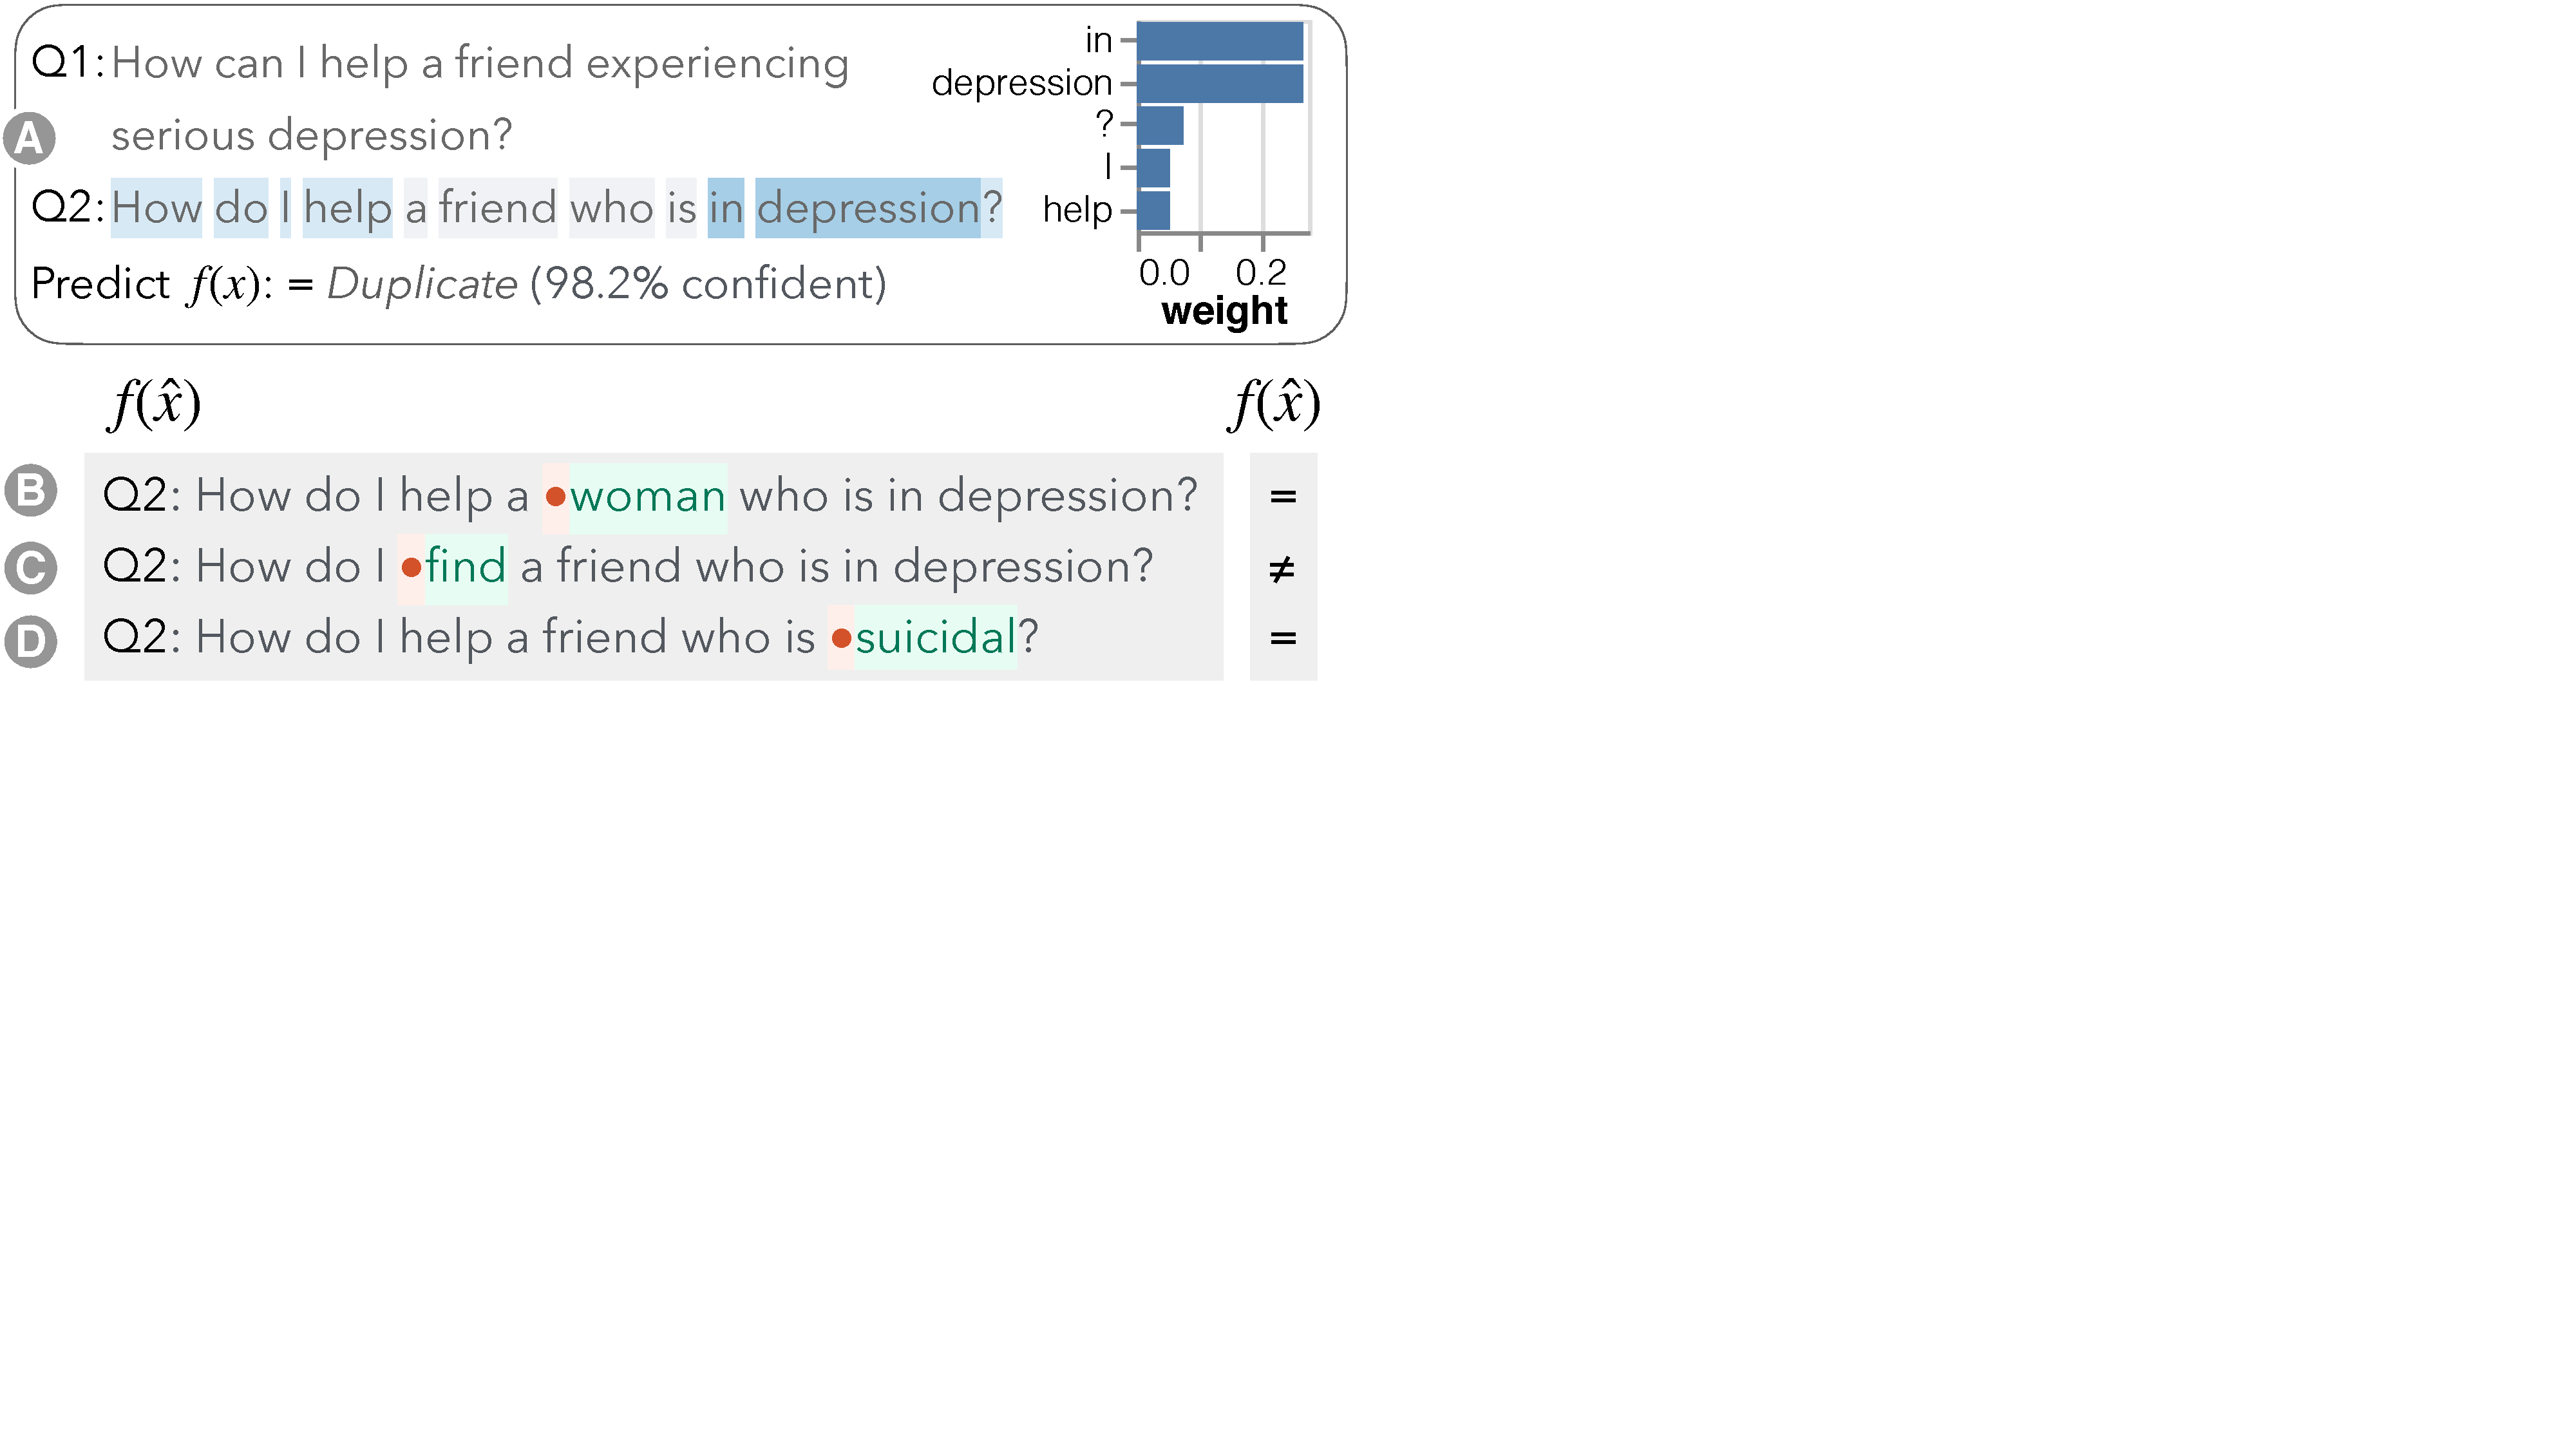
\includegraphics[trim={0 21cm 33cm 0cm},clip,width=1\columnwidth]{figures/explanation_v2.pdf}
\vspace{-15pt}
\caption{
(A) A \qqp instance where the model predicts ``duplicate'' ($=$) with 98.2\% confidence, as well as the SHAP weights for tokens in Q2.
%Counterfactual explanations complement SHAP with concrete, readable examples, \eg (C) depicts a surprising flipped prediction ($\neq)$ that was missed by SHAP.
Counterfactual explanations complement SHAP with concrete examples and surprising behaviors, \eg (C)
depicts an unexpected flipped prediction ($\neq)$, given the low SHAP weight of the perturbed token \swap{friend}{woman}.
}
\vspace{-10pt}
\label{fig:explanation}
\end{figure}

% \footnotetext{From BERT \qqp model: \url{https://huggingface.co/textattack/bert-base-uncased-QQP}}

%Such explanations have been elusive in NLP, despite evidence from social science research~\cite{miller} indicating that they may be more intuitive, or may complement feature attribution or attention maps. 
%Counterfactuals also naturally support model explanations, as ``explanations are sought in response to particular counterfactual cases or foils''~\cite{miller}.
%Popular feature importance attribution methods like SHAP~\cite{NIPS2017_7062} or LIME~\cite{Ribeiro2016WhySI} all retrieve token importance through masking, which can be viewed as a form of (incomplete) counterfactual.


%%%%%%%%%%%%%%%%%%%%%%%%%%%%%%%%%%%%%%%%%%%%%%%%%%%%%%%%%%%%
\begin{comment}
%%% Some useful comments from Miller's paper %%%
% about abnormality
people tend to ask questions about events or observations that they consider abnormal or unexpected from their own point of view people ask for explanations about events or observations that they consider abnormal or unexpected from their own point of view.

concepts such as abnormality could be used to infer likely foils.

People mostly ask for explanations of events that they find unusual or abnormal [77, 73, 69], and violation of normative behaviour is one such abnormality [73]. considered abnormal.

Abnormality clearly plays a role in explanation and interpretability. For explanation, it serves as a trigger for explanation, and is a useful criteria for explanation selection. For interpretability, it is clear that ‘normal’ behaviour will, on aggregate, be judged more explainable than abnormal behaviour.

The results showed participants provided explanations that are tailored to their expectations of what the hearer already knows, selecting single causes based on abnormal factors of which they believe the explainee is unaware; and that participants change their explanations of the same event when presenting to explainees with differing background knowledge

% about model interaction
individual users should require less explanation the more they interact with a system. First, because they will construct a better mental model of the system and be able to generalise its behaviour (effectively learning its model). Second, as they see more cases, they should become less surprised by abnormal phenomena, which as noted in Section 4.4.2, is a primary trigger for requesting explanations. An intelligent agent that presents — unprompted – an explanation alongside every decision, runs a risk of providing explanations that become less needed and more distracting over time

% about interactive explanation
I argue that, if we are to design and implement agents that can truly explain themselves, in many scenarios, the explanation will have to be interactive and adhere to maxims of communication, irrelevant of the media used. For example, what should an explanatory agent do if the explainee does not accept a selected explanation?

% attribution v.s. contrastive explanation
An important concept is the relationship between cause attribution and explanation. Extracting a causal chain and displaying it to a person is causal attribution, not (necessarily) an explanation. While a person could use such a causal chain to obtain their own explanation, I argue that this does not constitute giving an explanation. In particular, for most AI models, it is not reasonable to expect a lay-user to be able to interpret a causal chain, no matter how it is presented. Much of the existing work in explainable AI literature is on the causal attribution part of explanation — something that, in many cases, is the easiest part of the problem because the causes are well understood, formalised, and accessible by the underlying models. In later sections, we will see more on the difference between attribution and explanation, why existing work in causal attribution is only part of the problem of explanation, and insights of how this work can be extended to produce more intuitive explanations.
\end{comment}
%%%%%%%%%%%%%%%%%%%%%%%%%%%%%%%%%%%%%%%%%%%%%%%%%%%%%%%%%%%%


% \subsection{Foils to Feature Attribution Explanations}
A popular way of explaining NLP models is attributing importance weights to the input tokens, computed either from attention scores~\cite{wiegreffe2019attention} or by summarizing the model behavior on perturbed instances \cite{Ribeiro2016WhySI, NIPS2017_7062}.
Even if token scores really reflect their real importance to the model (\citet{pruthi2020learning} provide counter-examples), they can be too abstract for users to really understand model behavior~\cite{miller}. For example, while the explanation in Figure~\ref{fig:explanation}A indicates that the token ``help'' in Q2 is not very important, it's hard for users to grasp what that means without concrete examples, such as the one in Figure \ref{fig:explanation}B. 

Feature attribution methods are still useful as high level summaries, as the alternative of presenting a large number of counterfactuals would be overwhelming. One way to improve them with \sysname{} is by making them interactive, showing multiple counterfactuals that perturb the same span on-demand, a technique we explore in the next section. Here, we propose a complementary improvement: displaying a judicious selection of \sysname{} counterfactuals in addition to importance weights. 
Following \citet{miller}'s observation that people look for explanations that reveal \emph{unexpected} behavior, we select counterfactuals that violate the expectations set by the feature attributions, \ie examples where the \emph{real} change in prediction is large even though importance scores are low (Figure~\ref{fig:explanation}C) and examples where the change is small though importance scores are high (Figure~\ref{fig:explanation}D)\footnote{Details in Appendix \ref{appendix:exp_rank}}.
%TODO: Do we want to cut this line?
% This procedure also has the advantage of highlighting limitations of perturbations based on masking, used by popular packages such as LIME~\cite{Ribeiro2016WhySI} and SHAP~\cite{NIPS2017_7062}.


% While helpful as summaries, token scores may not reflect their real importance to the model, a limitation well known for attention \cite{pruthi2020learning} and inherent to perturbation-based methods relying exclusively on masking tokens, e.g. ``friend'' has near-zero weight in Figure \ref{fig:explanation}, even though \swap{friend}{woman} flips the prediction in \ref{fig:explanation}C (\swap{friend}{[MASK]} has no effect on the prediction).


% 	B. Problem 1: can lead to error if it's too abstract, provide an example where a non important feature really is not important, but should be. Cite social science: people like counterfactuals, people like foils, people like concrete (is this in social science? Lol)
%     Problem 2: relies on masking or attention, may not correspond to natural counterfactual cases


% Counterfactuals are essential for interpretability, as people seek for explanations through contrastive cases or ``foils.''~\cite{miller}.
% Because a large set of counterfactuals can be overwhelming, current techniques use feature attributions to summarize various local perturbations (\eg SHAP~\cite{NIPS2017_7062} or LIME~\cite{Ribeiro2016WhySI}).

% However, the resulting overview faces two challenges.
% First, feature weights can be too abstract for people to fully grasp.
% Without \swap{help}{find} in Figure~\ref{fig:explanation}B, an analyst viewing Figure~\ref{fig:explanation}A can hardly notice that the BERT \qqp model incorrectly assigns \remove{help} as a trivial feature.
% % see above for the actual quote. Did I interpret it correctly?
% Indeed, \citet{miller} argued that it may be unreasonable to expect a lay-user to be able to interpret an attribution, and that concrete foils are more intuitive.
% Second, feature attribution methods estimate weights by \emph{masking} words, which may not correspond to natural counterfactual cases involving \eg word substitutions.
% The usually overlooked gap can mislead analysts to over-generalize their perceived model behaviors.


% To address such issues, we present \sysname counterfactuals in addition to feature attributions.
% Following \citet{miller}'s observations that abnormal factors are more salient, we select counterfactuals that \emph{violate expectation}.
% That is, for each $\xp$, we compute the deviation of its \emph{actual} change of prediction from the \emph{expected} change, given the weights of perturbed features.
% We select $\xp$ that displays large prediction change, when small changes are expected. 
% In Figure~\ref{fig:explanation}C, \swap{friend}{woman} changes the prediction from \emph{Duplicate} to \emph{Non-Duplicate}, even though ``friend'' has low weight; 
% Conversely, we also include those with small changes, when large changes are expected.
% In Figure~\ref{fig:explanation}D, changing the important \remove{in depression} still results in \emph{Duplicate}.
% Computational details are in Appendix~\ref{appendix:exp_rank}.

% \subsection{User Evaluation}
% \label{subsec:exp_user_study}

\newcommand{\cshap}{\emph{\sysname-surprise}\xspace}
\newcommand{\crandom}{\emph{\sysname-random}\xspace}
\newcommand{\chuman}{\emph{Expert}\xspace}

\paragraph{User evaluation.} We study the scenario where an expert has access to a model and local explanations, and evaluate the \emph{additional} benefit of showing counterfactuals, i.e. whether they bring \emph{new} insights. 
We evaluate three ways of generating counterfactuals: (1) \crandom, a baseline where we show random \sysname{} counterfactuals, (2) \chuman, where two graduate students (non-participants) were given access to the model and instructed to create counterfactuals that are surprising given the associated SHAP scores, and (3) \cshap, which uses the selection procedure described in the previous paragraph.
%The authors manually checked that all counterfactuals were fluent and unambiguous.
% We aim to answer: does seeing counterfactuals bring new insights, or are counterfactuals redundant with manual analysis or explanations?

We recruited 13 participants (graduate students with experience in model explanations), and had them analyze the aforementioned \qqp model. In each round, users were shown an example, the model prediction, and a SHAP explanation, as in Figure \ref{fig:explanation}A. Users were instructed to create up to $10$ counterfactuals in order to better understand model behavior around the example, for which model predictions were given (users created $6$ on average). 
Finally, users were asked to simulate what the model would do on six counterfactuals, two from each condition (in random order). Counterfactuals where users make mistakes are preferable, as displaying these would add information that users do not already have.

% \paragraph{Setup.}
% We recruited 13 graduate students with experience in model explanations, and asked them to simulate the predictions of the aforementioned \qqp model on counterfactuals for 20 rounds.
% Intuitively, if the users are mistaken during the simulations, showing them such counterfactuals would add new information.
% In each round, the participants were given a base example, model prediction on it, and the SHAP weights, displayed as in Figure~\ref{fig:explanation}A.
% They could also create up to 10 counterfactuals to query model behaviors (they used around 6 chances.)
% Participants then simulated model predictions on six counterfactuals, two from each of the following conditions.
% We concluded the study with surveys on their query and simulation strategies.

% \paragraph{Conditions.} 
% We compare three types of counterfactuals:
% (1) \cshap, the \sysname-generated, abnormal counterfactuals, selected to complement SHAP; 
% (2) \crandom, the randomly selected \sysname counterfactuals; 
% (3) \chuman, the human-generated counterfactuals, in which two graduate students (not participants) played with the model, and each created one $\xp$ where the prediction was counter-intuitive according to the SHAP score on $x$.
% This is similar to hiring someone else to ``break the analysis'' with surprising examples.
%The authors manually checked that all counterfactuals were fluent and unambiguous.
% All the counterfactuals were close to the original examples, both in terms of the syntactic tree edit distance (0.97 in \cshap, to 1.25 in \chuman) and Levenshtein distance (around 0.2 in all conditions).
% \wts{remove Levenshtein here or add it to intrinsic evaluation part. this is what's used in MiCE.}

% \begin{comment}
\begin{figure}[t]
\centering
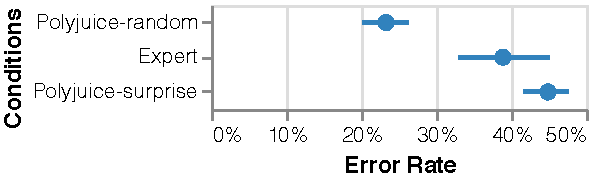
\includegraphics[width=1\columnwidth]{figures/err_rate.pdf}
\vspace{-15pt}
\caption{
Simulation error rates on counterfactuals. Higher error rates are better, indicating counterfactuals that would add more information to users if displayed.
}
\vspace{-10pt}
\label{fig:err_rate}
\end{figure}
% \end{comment}

\paragraph{Results.}
We present simulation error rates in Figure \ref{fig:err_rate}, where we see that humans can simulate model behavior on \cshap counterfactuals only slightly better than random guessing ($45\%\pm6\%$), i.e. these examples display model behavior that is surprising to users even after seeing explanations and creating their own counterfactuals. \chuman counterfactuals also had a high error rate, but at a much higher cost: generating these took 1.5--2 hours of expert labor, for $20$ instances.

While high error rate could be achieved with unrelated or nonsensical examples, all counterfactuals under evaluation were close to the original examples, when measured by syntatic tree edit distance ($\approx1.0$) or Levenshtein distance ($\approx0.2$), \cshap being the closest on both. An independent rater labeled $95\%$ of \cshap counterfactuals as ``likely written by a native speaker'', in contrast to $85\%$ for \chuman, indicating that experts sometimes resorted to ungrammatical or nonsensical sentences in order to find surprising behavior.

% Have to decide if it's worth keeping this paragraph
Qualitatively, the study participants tended to create counterfactuals by perturbing the token with the highest weights (84\% of counterfactuals perturbed tokens in the top 15\% quantile of weights), not gaining a real understanding of how the other tokens impact predictions. Participants also made a significant number of mistakes even for tokens they had inspected, e.g. a participant perturbed the example in Figure \ref{fig:explanation}A by replacing \swap{help}{play with}, which the model predicts as \emph{Non-Duplicate}. When faced with \swap{help}{find} in Figure \ref{fig:explanation}, they incorrectly assumed the behavior would be the same.

These results indicate that \sysname{} counterfactuals complement feature attribution explanations by displaying information that users often miss even after exploring the model behavior manually, \emph{beyond} explanations. Moreover, \sysname{} counterfactuals for this application were more surprising and fluent than \chuman, despite being computed automatically at no extra cost.

% All the counterfactuals were close to the original examples, both in terms of the syntactic tree edit distance (0.97 in \cshap, to 1.25 in \chuman) and Levenshtein distance (around 0.2 in all conditions).
% \wts{remove Levenshtein here or add it to intrinsic evaluation part. this is what's used in MiCE.}

% As a within-subject study, we compared the error rate of human simulations across the three conditions.
% Participants only did slightly better than random guess on \cshap cases, with error rate $e=45\%\pm6\%$.
% If presented, these counterfactuals should bring more insights than hiring an expert graduate student to create counterfactuals ($e=39\%\pm11\%$), and more effectively: each graduate student had to spend 1.5--2 hours to generate 20 ``abnormal'' counterfactuals. 
% \crandom cases can be easily simulated ($e=23\%\pm6\%$), indicating the importance of abnormal counterfactuals.

% Another graduate student rated the fluency of counterfactuals, and verified that the simulation failure was not due to nonsensical noise.
% Interestingly, the rater deemed more than 95\% counterfactuals to be likely written by native speakers in both \sysname conditions, but only 85\% for \chuman, indicating that humans wrote ungrammatical sentences in order to find puzzling behavior.

% Participants' manual analysis revealed that they mostly erred when they missed the inspection spot.
% They focused mostly on what SHAP explanations deemed important, and ignored what was unimportant --- 84\% of their querying counterfactuals perturbed the most important features in the instance.\footnote{Tokens with weights higher than the 85\% quantile of all the weights in the instance.}
% For example, they repeatedly perturbed ``depression'' in Figure~\ref{fig:explanation}A, and therefore had to guess when simulating Figure~\ref{fig:explanation}B.
% In their survey responses, 7 participants explicitly stated their focus on important features, confirming that feature attributions can lead to incomplete comprehension.

% There are also 24\% of the missed \cshap cases where participants only partially inspected the related pattern,\footnote{At least one of their queries perturbed the same spans as $\xp$, and query text overlaps with the $\xp$ for over 70\%.} and were misled by it --- ``followed similar examples I tried,'' as one subject articulated.
% They could not to imagine the model predicting \emph{Duplicate} on Figure~\ref{fig:explanation}B (\swap{help}{find}), when it predicted \emph{Non-Duplicate} on their query \exinline{How do I \swap{help}{play with}...?}
% The number dropped to $15\%$ for the \chuman condition, showing that \cshap found more bugs in spots that participants considered inspected.

% \subsection{Discussions}

% \sysname counterfactuals is preferable over hiring a second expert analyst: they help find more insights at lower annotation cost, with less ungrammatical changes, and help extend manual inspection more exhaustively.
% However, certain forms of explanation selection is necessary to overcome the obvious ones. 
% The abnormality is one useful criteria that aligns with humans' cognitive processes, but humans should also be able to drive the selection, and acquire concrete foils for any spans \emph{they} do not understand.
% For example, an analyst can \texttt{BLANK} ``friend'' in Q2 in Figure~\ref{fig:explanation}C, and observe the model's unstable behavior: it predicts \emph{Non-duplicate} when \remove{friend} is changed to \add{woman}, \add{professional}, but remains \emph{Duplicate} at \add{man}, \add{student}.
% We discuss the interactions in \S\ref{sec:err_analysis}.

% As \citet{miller} noted, individual users should require less explanation the more they interact with a system.
% The fact that \sysname can still complement users' mental models, even after they see the feature attributions and manually inspect the model, indicates that the gain can be more prominent when such explanation and model access is not available. 
% We envision that the abnormality selection can also help select standalone explanations, if the expectation is instead estimated without feature attribution explanations (\eg he distance in the latent space~\cite{reimers-2019-sentence-bert}).
% We defer the exploration to future work.
